% !TeX root = f44_shortreport_schmitt_kleinbek.tex
\section{Measurements Log and Evaluation}
\subsubsection{First Part: Spectroscopy of the Zeeman effect}
In the first part of the experiment, the Zeeman effect was investigated using the red cadmium line, which ist formed at the transition from $^1\text{D}_2\rightarrow ~^1\text{P}_1$.\\

To this end, it should first be examined whether a hystheresis effect occurs with the magnets used.
For this purpose, three measurements were performed with a Hall probe each with increasing and decreasing field strength in the relevant range and the results for $B_\text{inc}$ and $B_\text{dec}$ were averaged.
In Figure \ref{fig:hystheresis} you see the results of this measurement.
\begin{figure}[ht]
\centering
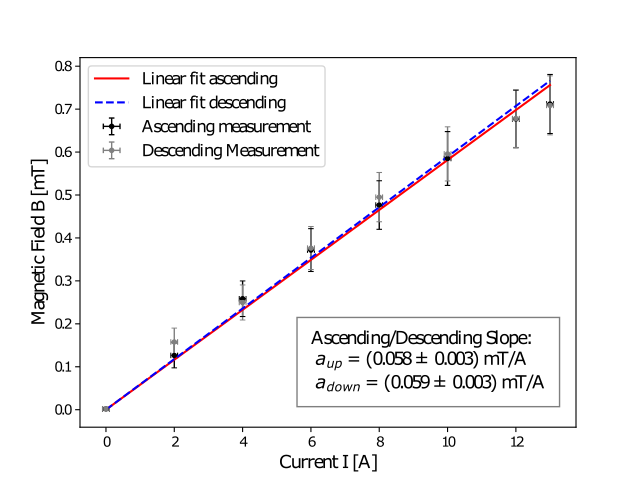
\includegraphics[scale=.55]{images//hystheresis.png}
\caption{Comparison of the magnetic field strength with increasing and decreasing current strength}
\label{fig:hystheresis}
\end{figure}
You can see that there is a small difference between the measurements, but the fit reveals that this difference is within the error, which is why in our case there is no significant effect.\\

Next, the Zeeman effect should be qualitatively investigated in longitudinal and transverse direction.
For this purpose, we used the structure shown in figure \ref{fig:structure}.
\begin{figure}[ht]
\centering
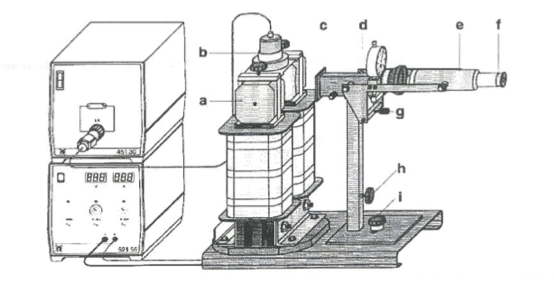
\includegraphics[scale=.9]{images//structure.png}
\caption{Experimental set-up: a) Pole pieces of the magnet, b) Cd lamp, c) Red light filter, d) Lummer-Gehrcke Plate, e) Telescope, f) Eyepiece, g) Height adjustment for the telescope, h) Locking screw for the telescope holder, i) Locking screw for the base plate. \cite{leaflets}}
\label{fig:structure}
\end{figure}
The most important element of this construction is the Lummer-Gehrcke plate with almost plane-parallel surfaces.
If light enters the plate trough a prism with an angle of incidence of $\beta$, it is reflected inside the plate.
After each reflection some light is refracted at the surface, which is focused with the help of a lens and brought to interference.\\
If the gait difference meets the conditions
\begin{align}
\Delta_i = 2d\sqrt{n_i^2-1} = k \lambda
\end{align}
constructive interference with the gear difference $\Delta=\Delta_1-\Delta_2$ is obtained. Therefore the refractive index is $n=n_2$ and $n_1\approx\num{1}$, the thickness of the plate is $d$ and the interference order is $k$.
The reflection angle $\alpha$ within the plate is assumed to be approximately $\ang{90}$, resulting in near total reflection within the plate.\\
Our interference pattern of the Lummer-Gehrcke plate for a transversal image can be seen in Figure \ref{fig:interference}.
\begin{figure}[ht]
\centering
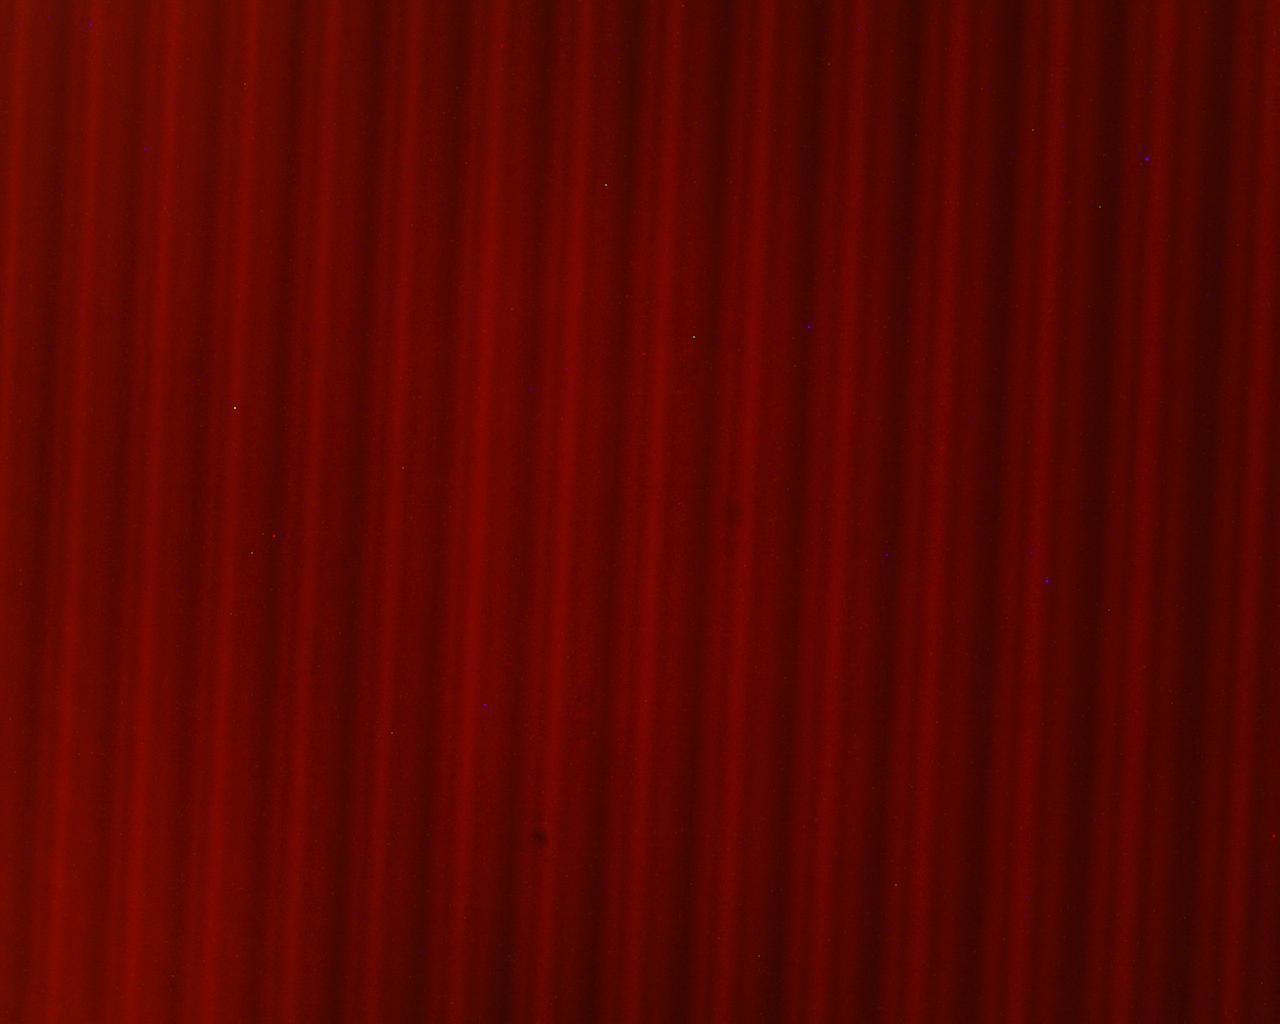
\includegraphics[scale=.14]{images//interference.jpg}
\caption{Zeeman effect with $\SI{13}{\ampere}$}
\label{fig:interference}
\end{figure}
The quantitative results from the observation of the Zeeman effect should next be used to determine Bohr's magneton.
For this purpose, the images from the first test section were plotted in Python and fitted with a Gaussian function.
This gave us the positions and width of the interference lines in pixels for each measurement with $I =\SIlist{9;11;13}{\ampere}$.
\begin{figure}[ht]
\centering
\begin{subfigure}{.24\textwidth}
\centering
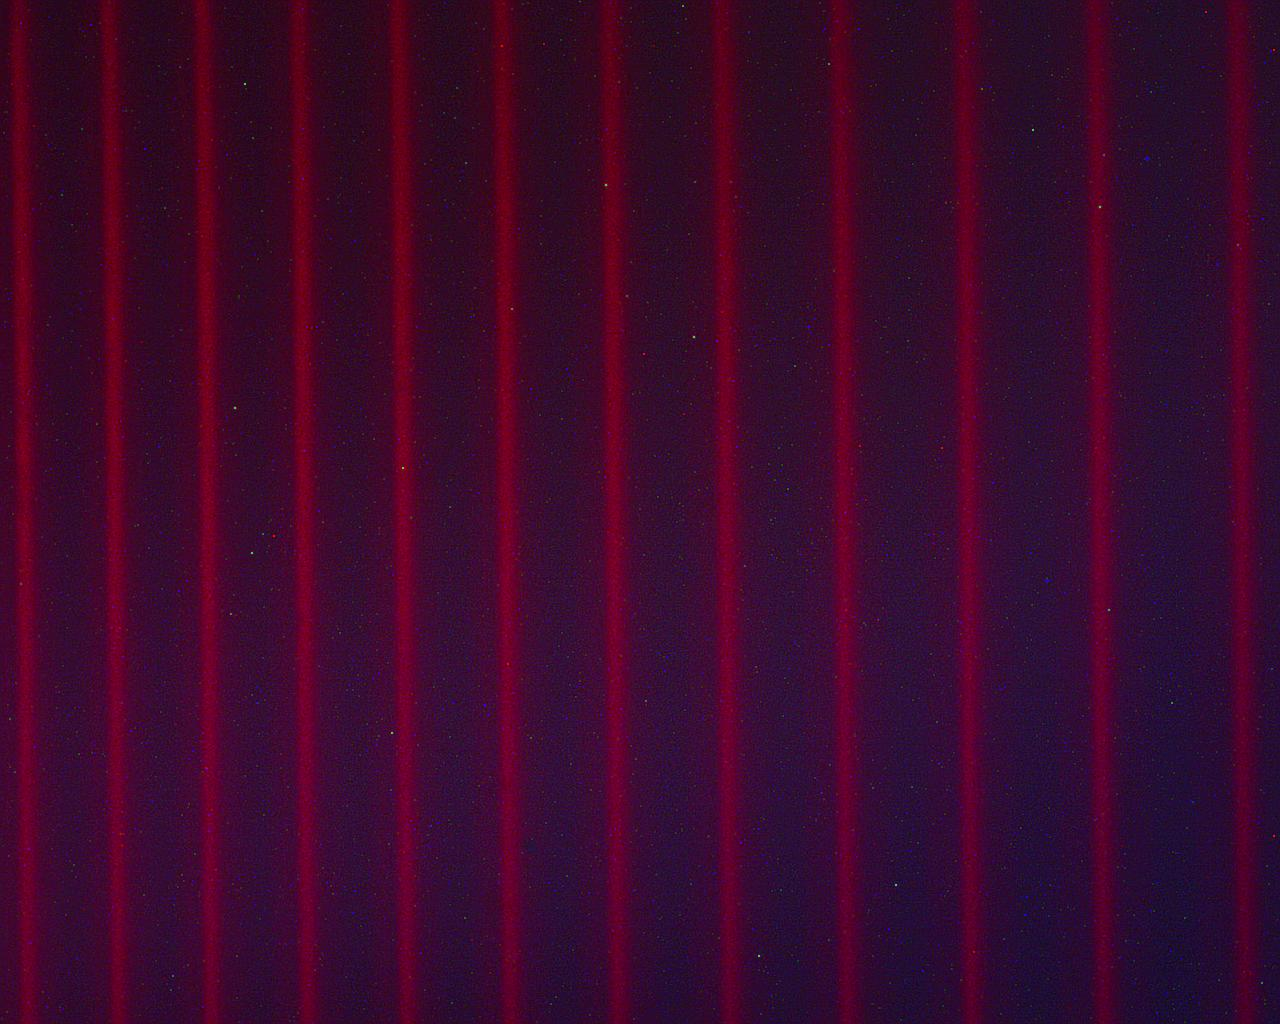
\includegraphics[scale=.115]{images//pi.jpg}
\caption{$\pi$-lines}
\end{subfigure}
\begin{subfigure}{.24\textwidth}
\centering
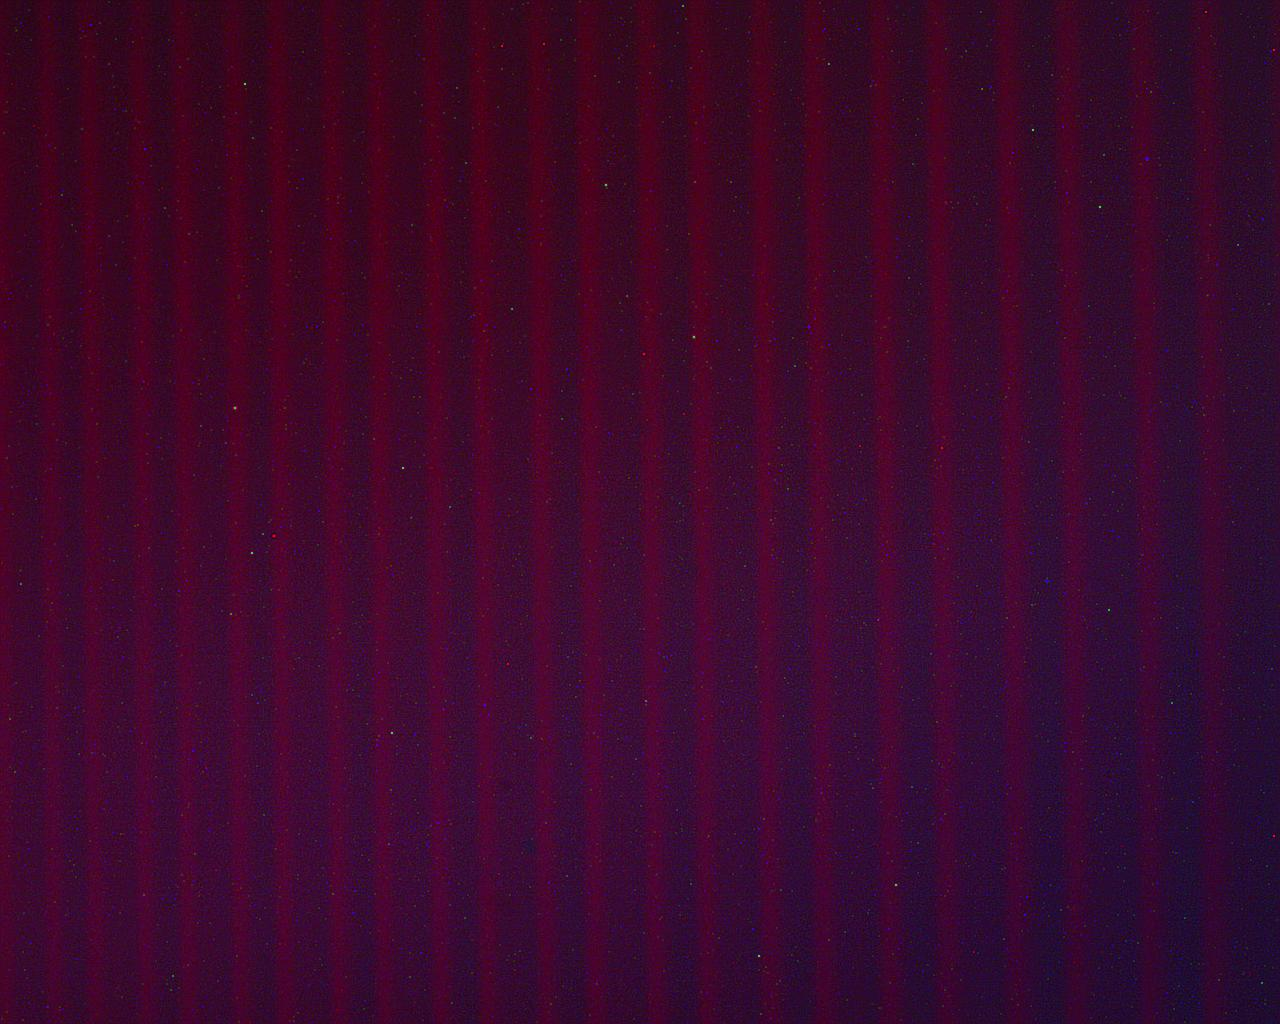
\includegraphics[scale=.115]{images//sigma.jpg}
\caption{$\sigma$-lines}
\end{subfigure}
\caption{Interference with $\SI{11}{\ampere}$}
\label{fig:pisigma}
\end{figure}
The orders of the $\pi$-lines were plotted against the position in pixels and provided with a second-order polynomial fit.
With the help of this fit the orders of the $\sigma$-lines were determined.\\

In order to determine Bohr's magneton, we consider the distance between the $\pi$- and $\sigma$-lines, which can identify the wavelengths as $\lambda$ and $\lambda + \delta \lambda$.
For $\delta \lambda$ from the measurement
\begin{align}
\delta \lambda = \frac{\delta k}{\Delta k}\cdot\Delta \lambda = \delta k \cdot\Delta \lambda
\end{align}
with $\Delta k$ the order difference between two $\pi$-lines, $\delta k$ the order difference between $\pi$- and $\sigma$-lines and $\Delta\lambda$ determined by
\begin{align}
\Delta \lambda = \frac{\lambda^2}{2d \sqrt{n^2 -1}}.
\end{align}
Thus for $\delta\lambda$ depending on $\delta k$ the equation
\begin{align}
\delta \lambda = \delta k \cdot\frac{\lambda^2}{2d \sqrt{n^2 -1}}
\end{align}
results with $n = \num{1.457}$ and $d = \SI{4.04}{\milli\meter}$.
For this measurement $\lambda$ is the wavelength of the red cadmium line, which we determined as $\lambda_\text{Cd} = \SI{643.8(29)}{\nano\meter}$ in the second part of the experiment.\\
Using the energy difference $E_\text{pot}$ of two wavelengths
\begin{align}
\Delta E_{pot} = hc \left(\frac{1}{\lambda_1}-\frac{1}{\lambda_2}\right) \approx hc \cdot\frac{\delta \lambda}{\Delta \lambda}
\end{align}
and equates it with the energy difference of the associated energy levels (see Eq. \ref{eq:energydiff}), then one obtains 
\begin{align}
\mu_\text{B} = \frac{hc}{2Bd \sqrt{n^2 -1}}\cdot\delta k.
\end{align}
\begin{table}[ht]
\centering
\begin{tabular}{CCC}
\toprule
I\, [\si{\ampere}] & B\, [\si{\tesla}] & \mu_\text{B}\, [\SI{e-24}{\joule\per\tesla}]\\
\midrule
\num{9} & \num{0.527(19)} & \num{10.1(15)}\\
\num{11} & \num{0.644(23)} & \num{9.8(15)}\\
\num{13} & \num{0.761(27)} & \num{9.7(8)}\\
\bottomrule
\end{tabular}
\caption{Bohr's magneton for each current}
\label{tab:bohr}
\end{table}
In our experiment, a Bohr's magneton of
\begin{align*}
\mu_\text{B}=\SI{9.7(8)e-24}{\joule\per\tesla}
\end{align*}
is obtained, while the literature value is $\mu_\text{B}=\SI{9.274e-24}{\joule\per\tesla}$ and the two values overlap in the 1$\sigma$-range.\\
The error results from error propagation on the standard deviation analogous to the standard deviation of the Gaussian peaks in Fig. \ref{fig:gaussian} builds up.
\begin{figure}[ht]
\centering
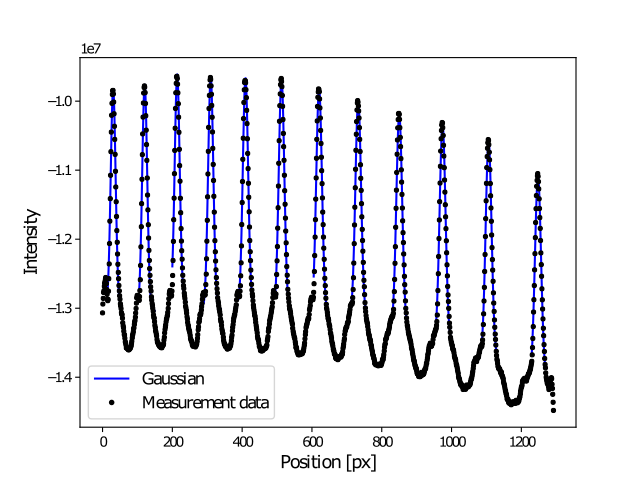
\includegraphics[scale=.55]{images//gaussian.png}
\caption{$\pi$-lines with $\SI{11}{\ampere}$}
\label{fig:gaussian}
\end{figure}

\subsubsection{Second Part: Precision spectroscopy}
In the second part of the experiment, the wavelengths of two lines of the cadmium spectrum were to be determined.\\

A Czerny-Turner spectrometer with a neon lamp as a reference was used for this purpose.\\
The Czerny-Turner spectrometer allows the spectral acquisition of the wavelengths of incoming light with the aid of grating.
The light entering through an opening is focused trough a concave mirror onto the grating, where it is spectrally split and then reflected by another mirror so that the built-in CCD camera is in the focal plane of the spectrum.\\

First, we determined the position of the peaks in the neon spectrum in the range around $\SI{640}{\nano\meter}$ in a reference measurement.
The peaks in the spectrum image were provided with Gaussian fits to determine the position and assigned to the appropriate wavelengths (see Fig. \ref{fig:spectrum}).
\begin{figure}[ht]
\centering
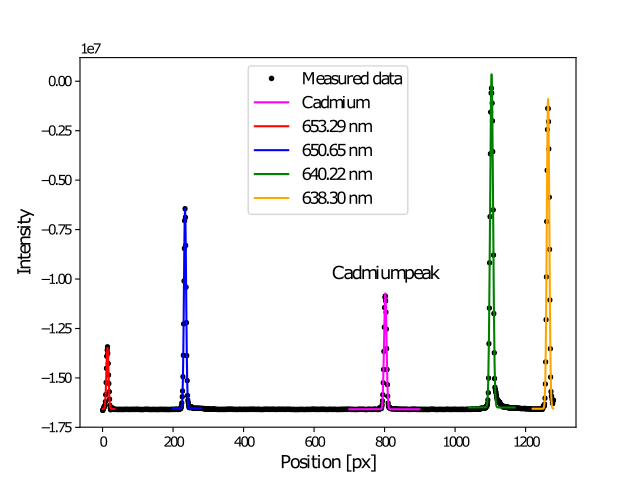
\includegraphics[scale=.55]{images//spectrum.png}
\caption{Spectrum of Cadmium and Neon}
\label{fig:spectrum}
\end{figure}

Then the wavelength of the Neon peaks against their position was plotted in pixels (see Fig. \ref{fig:position}) and fitted with a linear function.
The standard deviation of the Gaussian Distribution was used as error.
\begin{figure}[ht]
\centering
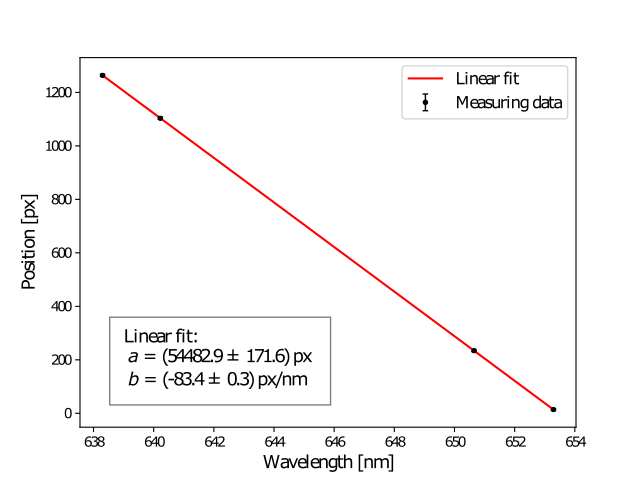
\includegraphics[scale=.55]{images//position.png}
\caption{Position as function of the wavelength}
\label{fig:position}
\end{figure}
In a second measurement, we recorded the spectrum of the cadmium lamp with the same settings and also determined the position of the peaks using a Gaussian fit.
From the fit of the first measurement we could then calculate the wavelengths of the two visible lines.\\
For the strong cadmium line we obtained a wavelength of
\begin{align*}
\lambda_\text{Cd}=\SI{643.8(29)}{\nano\meter}.
\end{align*}
Unfortunately, we were no longer able to break up another weak line.
Nevertheles, it can be assumed that Xenon is to be seen as gaseous impurity or Tungsten as electrode material.